\documentclass[11pt,a4paper]{article}

\usepackage[margin=2.4cm]{geometry}
\usepackage[utf8]{inputenc}
\usepackage{lmodern}
\usepackage[T1]{fontenc}
\usepackage{amsmath,amssymb,amsfonts,amsthm}
\usepackage{mathtools}
\usepackage{booktabs}
\usepackage{array}
\usepackage{enumitem}
\usepackage{graphicx}
\usepackage{listings}
\usepackage{xcolor}
\usepackage{hyperref}
\hypersetup{colorlinks=true, linkcolor=blue, citecolor=blue, urlcolor=blue}

\lstset{
  language=Python,
  basicstyle=\ttfamily\footnotesize,
  keywordstyle=\bfseries,
  commentstyle=\itshape\color{gray},
  breaklines=true,
  frame=single,
  columns=fullflexible,
  keepspaces=true,
  showstringspaces=false,
  aboveskip=0.6em,
  belowskip=0.6em,
}

\theoremstyle{plain}
\newtheorem{theorem}{Teorema}
\newtheorem{lemma}[theorem]{Lema}
\newtheorem{proposition}[theorem]{Proposici\'on}
\newtheorem{corollary}[theorem]{Corolario}

\theoremstyle{definition}
\newtheorem{definition}{Definici\'on}
\newtheorem{remark}{Observaci\'on}
\newtheorem{assumption}{Hip\'otesis}

\newcommand{\vect}[1]{\boldsymbol{#1}}
\newcommand{\matr}[1]{\mathbf{#1}}
\newcommand{\R}{\mathbb{R}}
\newcommand{\N}{\mathbb{N}}
\newcommand{\softplus}{\operatorname{softplus}}
\newcommand{\erf}{\operatorname{erf}}
\newcommand{\norm}[1]{\left\lVert #1 \right\rVert}
\newcommand{\abs}[1]{\left\lvert #1 \right\rvert}
\DeclareMathOperator{\diag}{diag}
\DeclareMathOperator{\Cov}{Cov}
\DeclareMathOperator{\sgn}{sgn}
\DeclareMathOperator{\supp}{supp}
\DeclareMathOperator*{\esssup}{ess\,sup}

\title{Un forward anal\'itico \emph{diferenciable} para el CRB de la
c\'amara de esquina activa\\[4pt]
\large Del render rasterizado a derivadas cerradas (Camino A)}
\author{Obstacle Detection Study}
\date{\today}

\begin{document}
\maketitle

\begin{abstract}
Este documento explica, en orden pedag\'ogico, c\'omo construimos un
\textbf{forward anal\'itico diferenciable} de la faceta oculta para el c\'alculo
del Cram\'er--Rao (CRB), con \textbf{derivadas parciales cerradas}, sin modificar
el simulador rasterizado existente (\texttt{pyerti.py},
\texttt{simulation\_polar\_clean.ipynb}, \texttt{crb\_polar\_functions.py}).
Partimos del forward \emph{actual} --- un render rasterizado cuyas fuentes de
no diferenciabilidad (cuantizaci\'on temporal con \texttt{ceil}, ocultamiento
por umbral duro, \emph{clamps} \texttt{max}$(0,\cdot)$, dep\'osito en p\'ixeles y
bins enteros) impiden escribir $\partial g/\partial\vect{\psi}$ en forma
cerrada --- y lo reemplazamos, pieza por pieza, por an\'alogos suaves de clase
$C^\infty$: la masa de Dirac en un bin se convierte en la integral anal\'itica de
un pulso gaussiano (diferencia de $\erf$), el ocultamiento por umbral en una
sigmoide de penumbra, y los \emph{clamps} en \emph{softplus}. Las derivadas se
obtienen \textbf{simb\'olicamente} con \texttt{sympy} (an\'alogo al Mathematica
del \emph{writeup}) y se validan contra diferencias finitas del mismo forward
suave, con error m\'aximo relativo $\sim\!5\times10^{-10}$. El c\'odigo est\'a en
\texttt{crb\_analytic\_forward.py} y la validaci\'on en
\texttt{validate\_analytic\_forward.py}.
\end{abstract}

\tableofcontents
\bigskip\hrule\bigskip

%==============================================================================
\section{Punto de partida: el forward rasterizado y por qu\'e no es diferenciable}
\label{sec:partida}
%==============================================================================

El c\'alculo actual del CRB (documentado en \texttt{sustento\_teorico\_crb.tex})
usa como forward el simulador de transporte de luz \texttt{simulation} (motor
\texttt{pyerti.py}). Para una pose $\vect{\psi}=(\rho,\varphi,h)$ produce un cubo
transitorio esperado $y\in\R^{H\times W\times T}$ (p\'ixeles SPAD $\times$ bins de
tiempo), y se forma $g=\operatorname{vec}(y+b)$ con fondo $b>0$.

El simulador acumula, para cada tri\'angulo del \emph{mesh} de centro
$\vect{c}$ y cada muestra de piso $\vect{p}_f$, una contribuci\'on de la forma
(v\'ease \texttt{pyerti.py}, l\'ineas $\sim$278--312):
\begin{equation}
    \Delta y
    \;\propto\;
    I_{\mathrm{laser}}\, A\,
    \frac{[\hat{\vect n}\!\cdot\!\hat{\vect u}_1]_+\,
          [\hat{\vect n}\!\cdot\!\hat{\vect u}_2]_+\,
          [\hat{\vect n}_l\!\cdot\!\hat{\vect u}_3]_+\,
          [\hat{\vect n}_f\!\cdot\!\hat{\vect u}_4]_+}
         {4\pi^2\, d_1^2\, d_2^2},
    \label{eq:raster-dy}
\end{equation}
depositada \'unicamente en el bin entero de llegada
\begin{equation}
    j \;=\; \left\lceil \frac{d_1+d_2}{c\,\Delta t} \right\rceil ,
    \qquad d_1=\|\vect{p}_l-\vect{c}\|,\quad d_2=\|\vect{p}_f-\vect{c}\|,
    \label{eq:raster-ceil}
\end{equation}
y solo para los p\'ixeles \emph{no ocluidos}, seleccionados por la m\'ascara dura
\begin{equation}
    \texttt{noc}
    \;=\;
    \bigl(\texttt{xint}\ \text{finito}\bigr)\ \land\ (\texttt{xint}>0),
    \qquad
    \texttt{xint}=-b/m ,
    \label{eq:raster-noc}
\end{equation}
donde $m,b$ definen la recta faceta$\to$p\'ixel en el plano $XY$.

\begin{remark}[Por qu\'e $\partial g/\partial\vect{\psi}$ no existe en forma cerrada]
Tres operaciones de \eqref{eq:raster-dy}--\eqref{eq:raster-noc} son
\textbf{no diferenciables}:
\begin{enumerate}[nosep]
    \item \textbf{Cuantizaci\'on temporal} \eqref{eq:raster-ceil}: la funci\'on
    $\lceil\cdot\rceil$ es constante a trozos con saltos unitarios. Su derivada
    es cero casi en todas partes y una \emph{delta} en los saltos: al mover
    $\vect{\psi}$, la masa salta discretamente de un bin al siguiente.
    \item \textbf{Ocultamiento por umbral} \eqref{eq:raster-noc}: la indicatriz
    $\mathbf{1}\{\texttt{xint}>0\}$ es un Heaviside muestreado; su derivada es
    una delta en la frontera iluminado/sombra.
    \item \textbf{\emph{Clamps}} $[\,\cdot\,]_+=\max(0,\cdot)$ en el
    \emph{foreshortening}: continuos pero no derivables en $0$ (codo).
\end{enumerate}
Adem\'as el dep\'osito en \'indices enteros de p\'ixel/bin es intr\'insecamente
discreto. Por eso el pipeline vigente aproxima el Jacobiano por
\textbf{diferencias finitas} centrales sobre \emph{todos} los bins, usa un fondo
$b$ y un piso $\varepsilon$ (\texttt{fisher\_eps}) para que $1/g$ sea finito, y
debe elegir con cuidado los pasos $\delta$ (p.\,ej.\ $\delta\rho=0.01$\,m,
$\delta\varphi=0.5^\circ$, $\delta h=0.01$\,m). Este es el objeto que queremos
\emph{volver diferenciable}.
\end{remark}

%==============================================================================
\section{El modelo continuo del \emph{writeup}}
\label{sec:continuo}
%==============================================================================

El \emph{writeup} de la c\'amara de esquina activa (Seidel \emph{et al.})
parte de un modelo \textbf{continuo}. Con la faceta oculta puntual en
$\vect{p}_s=[\rho\cos\varphi,\ \rho\sin\varphi,\ h]$ y normal
$\hat{\vect n}_s=[-\cos\varphi,-\sin\varphi,0]$, l\'aser en $\vect{p}_l$
(normal $\hat{\vect n}_l$), c\'amara en $\vect{p}_c$ y punto de piso
$\vect{p}_f$ (normal $\hat{\vect n}_f$), la luz saliente en el instante $t$ es
(ec.~1 del \emph{writeup})
\begin{equation}
    L_h(\vect{p}_f,t)
    =
    \frac{\alpha\, H(\pi+\theta-\varphi)\,
          f(\vect{p}_c,\vect{p}_s,\vect{p}_l,\vect{p}_f)\,
          s\!\left(t-\tfrac{\|\vect{p}_s-\vect{p}_l\|+\|\vect{p}_s-\vect{p}_f\|}{c}\right)}
         {8\pi^3\,\|\vect{p}_c-\vect{p}_f\|^2\,
          \|\vect{p}_s-\vect{p}_l\|^2\,\|\vect{p}_s-\vect{p}_f\|^2},
    \label{eq:Lh}
\end{equation}
con $s(\cdot)$ el pulso, $H$ el escal\'on de Heaviside, $\alpha$ el albedo, y
$f$ el \emph{foreshortening} (producto de cinco cosenos, ec.~2):
\begin{equation}
    f
    =
    \frac{\hat{\vect n}_f\!\cdot\!(\vect{p}_c-\vect{p}_f)}{\|\vect{p}_c-\vect{p}_f\|}\,
    \frac{\hat{\vect n}_f\!\cdot\!(\vect{p}_s-\vect{p}_f)}{\|\vect{p}_f-\vect{p}_s\|}\,
    \frac{\hat{\vect n}_s\!\cdot\!(\vect{p}_f-\vect{p}_s)}{\|\vect{p}_f-\vect{p}_s\|}\,
    \frac{\hat{\vect n}_s\!\cdot\!(\vect{p}_l-\vect{p}_s)}{\|\vect{p}_l-\vect{p}_s\|}\,
    \frac{\hat{\vect n}_l\!\cdot\!(\vect{p}_s-\vect{p}_l)}{\|\vect{p}_l-\vect{p}_s\|}.
    \label{eq:foreshortening}
\end{equation}
La tasa de Poisson de la medici\'on $q=(i,j)$ (p\'ixel $i$, bin $j$) es la
integral sobre el p\'ixel y el bin (ec.~3):
\begin{equation}
    y_q
    =
    \int_{(j-1)\Delta t}^{j\Delta t}\!\!\int_{\vect{p}\in P_i}
    L_h(\vect{p}_f,t)\,d\vect{p}\,dt,
    \qquad
    g_q=y_q+b_q,\quad b_q>0.
    \label{eq:yq}
\end{equation}
El \emph{writeup} deriva $\partial y_q/\partial\Psi_m$ \emph{bajo el integrando}
con Mathematica (ecs.~9--11). Nuestro objetivo es reproducir esa idea con un
forward propio, expl\'icito y diferenciable en c\'odigo.

%==============================================================================
\section{Volviendo la funci\'on diferenciable, paso a paso}
\label{sec:suave}
%==============================================================================

Construimos un forward de \textbf{faceta puntual} que eval\'ua directamente el
integrando de \eqref{eq:Lh} sobre una malla fija de p\'ixeles de piso
$\{\vect{p}_{f,i}\}$ y una rejilla fija de bins $\{[t^{(j)}_{\mathrm{lo}},
t^{(j)}_{\mathrm{hi}}]\}$, sustituyendo cada operaci\'on no diferenciable por su
an\'alogo suave. Sea $\vect{p}_s(\vect{\psi})=[\rho\cos\varphi,\rho\sin\varphi,h]$.

\subsection{(i) Binning temporal: de \texttt{ceil} a una diferencia de \texorpdfstring{$\erf$}{erf}}
\label{sec:erf}
Esta es \textbf{la pieza central}. En el rasterizador toda la intensidad de un
p\'ixel se deposita en un \emph{\'unico} bin \eqref{eq:raster-ceil}: es una masa
de Dirac en $t_0(\vect{\psi})$, con
\begin{equation}
    t_0(\vect{\psi})
    =
    \frac{\|\vect{p}_s-\vect{p}_l\|+\|\vect{p}_s-\vect{p}_f\|}{c}.
    \label{eq:tof}
\end{equation}
Su an\'alogo suave es un \textbf{pulso gaussiano de \'area unitaria} centrado en
$t_0$,
\begin{equation}
    s(t)
    =
    \frac{1}{\tau\sqrt{2\pi}}\,
    \exp\!\left(-\frac{(t-t_0(\vect{\psi}))^2}{2\tau^2}\right),
    \qquad
    \int_{-\infty}^{\infty} s(t)\,dt = 1,
    \label{eq:pulse}
\end{equation}
de modo que, al sumar sobre bins, se recupera la masa total (la ``intensidad''
del rasterizador) pero de forma $C^\infty$. La integral del pulso sobre el bin
$[t_{\mathrm{lo}},t_{\mathrm{hi}}]$ es \textbf{cerrada}: con el cambio
$u=(t-t_0)/(\sqrt2\,\tau)$,
\begin{equation}
    \boxed{\;
    S_j(\vect{\psi})
    =
    \int_{t^{(j)}_{\mathrm{lo}}}^{t^{(j)}_{\mathrm{hi}}} s(t)\,dt
    =
    \frac{1}{2}
    \left[
        \erf\!\left(\frac{t^{(j)}_{\mathrm{hi}}-t_0(\vect{\psi})}{\sqrt2\,\tau}\right)
        -
        \erf\!\left(\frac{t^{(j)}_{\mathrm{lo}}-t_0(\vect{\psi})}{\sqrt2\,\tau}\right)
    \right].
    \;}
    \label{eq:erf-bin}
\end{equation}
La funci\'on $\erf$ es entera (anal\'itica en todo $\R$), de modo que $S_j$ es
$C^\infty$ en $\vect{\psi}$ a trav\'es de $t_0(\vect{\psi})$. Esto sustituye el
salto discreto del $\lceil\cdot\rceil$ por una transici\'on suave: al mover
$\vect{\psi}$, la masa se traspasa \emph{gradualmente} entre bins vecinos. El
par\'ametro $\tau$ (desviaci\'on est\'andar del pulso, en segundos) fija el ancho
temporal; por defecto $\tau=\Delta t=3.9\times10^{-10}$\,s.

\subsection{(ii) Ocultamiento: de umbral duro a sigmoide de penumbra}
\label{sec:vis}
La m\'ascara dura \eqref{eq:raster-noc} se define a partir de \texttt{xint}, la
coordenada $x$ donde el segmento faceta$\to$p\'ixel cruza el eje $y=0$. La
mantenemos \textbf{en forma cerrada} como funci\'on de borde (distancia firmada al
plano de ocultamiento):
\begin{equation}
    d_{\mathrm{edge}}(\vect{\psi},\vect{p}_f)
    =
    s_x - s_y\,\frac{s_x-p_x}{s_y-p_y},
    \qquad
    s_x=\rho\cos\varphi,\ \ s_y=\rho\sin\varphi,
    \label{eq:dedge}
\end{equation}
que coincide exactamente con el \texttt{xint} del rasterizador pero es suave en
$\vect{\psi}$ (salvo la recta $s_y=p_y$, tratada como l\'imite). El Heaviside
$\mathbf{1}\{d_{\mathrm{edge}}>0\}$ se reemplaza por una \textbf{sigmoide}
\begin{equation}
    \boxed{\;
    \mathrm{vis}(\vect{\psi},\vect{p}_f)
    =
    \sigma\!\bigl(\kappa\,d_{\mathrm{edge}}\bigr)
    =
    \frac{1}{1+e^{-\kappa\, d_{\mathrm{edge}}(\vect{\psi},\vect{p}_f)}}
    \;\in(0,1),
    \;}
    \label{eq:sigmoid}
\end{equation}
donde $\kappa>0$ es el \textbf{ancho de penumbra}: la transici\'on
sombra$\to$luz ocurre en una banda de semi-anchura $\sim 1/\kappa$ (metros) en la
coordenada de cruce. Cuando $\kappa\to\infty$ se recupera el Heaviside. Por
defecto $\kappa=60$ (penumbra $\sim1.7$\,cm, comparable al tama\~no de p\'ixel).

\subsection{(iii) \emph{Foreshortening}: de \texorpdfstring{$\max(0,\cdot)$}{max(0,.)} a \emph{softplus}}
\label{sec:softplus}
Cada coseno $c_k$ de \eqref{eq:foreshortening} puede ser negativo (cara opuesta);
el rasterizador aplica $[\,c_k\,]_+=\max(0,c_k)$, no derivable en $c_k=0$. Lo
reemplazamos por la \textbf{\emph{softplus}}
\begin{equation}
    \softplus_\beta(x)
    =
    \frac{1}{\beta}\log\!\bigl(1+e^{\beta x}\bigr),
    \qquad
    \softplus_\beta(x)\xrightarrow[\beta\to\infty]{}\max(0,x),
    \label{eq:softplus}
\end{equation}
cuya derivada es la sigmoide $\sigma(\beta x)\in(0,1)$, de modo que el codo se
suaviza en una escala $\sim1/\beta$. El \emph{foreshortening} suave es
\begin{equation}
    f_{\mathrm{smooth}}(\vect{\psi},\vect{p}_f)
    =
    \prod_{k=1}^{5}\softplus_\beta\!\bigl(c_k(\vect{\psi},\vect{p}_f)\bigr).
    \label{eq:f-smooth}
\end{equation}
Por defecto $\beta=50$ (ancho de codo $\sim0.02$). Las distancias
$\|\cdot\|=\sqrt{\langle\cdot,\cdot\rangle}$ ya son $C^\infty$ mientras no se
anulen (garantizado por la geometr\'ia: $\vect{p}_s\neq\vect{p}_l,\vect{p}_f$).

\subsection{(iv) Ensamblado de \texorpdfstring{$g(\vect{\psi})$}{g(psi)}}
\label{sec:ensamble}
Reuniendo \eqref{eq:erf-bin}, \eqref{eq:sigmoid} y \eqref{eq:f-smooth}, la tasa
esperada en la medici\'on $q=(i,j)$ es el producto
\begin{equation}
    \boxed{\;
    y_q(\vect{\psi})
    =
    \underbrace{\frac{\alpha\,G\;\mathrm{vis}(\vect{\psi},\vect{p}_{f,i})\,
                      f_{\mathrm{smooth}}(\vect{\psi},\vect{p}_{f,i})}
                     {8\pi^3\,\|\vect{p}_c-\vect{p}_{f,i}\|^2\,
                      \|\vect{p}_s-\vect{p}_l\|^2\,\|\vect{p}_s-\vect{p}_{f,i}\|^2}}
                     _{\textstyle A_i(\vect{\psi})\ \text{(amplitud espacial)}}
    \;\cdot\;
    \underbrace{S_j(\vect{\psi})}_{\textstyle \text{pulso en el bin}} ,
    \;}
    \label{eq:yq-smooth}
\end{equation}
con $G$ una ganancia global (potencia de l\'aser $\times$ escala de conteo) y
\begin{equation}
    g_q(\vect{\psi}) = y_q(\vect{\psi}) + b,
    \qquad b=0.1 .
    \label{eq:g-smooth}
\end{equation}
El fondo $b>0$ cumple el mismo papel que en el \emph{writeup}: mantiene $1/g_q$
finito \textbf{sin} necesidad de un piso $\varepsilon$ artificial. Cada factor de
\eqref{eq:yq-smooth} es $C^\infty$ en $\vect{\psi}=(\rho,\varphi,h)$, luego $g_q$
lo es. Esto est\'a implementado en \texttt{crb\_analytic\_forward.py}
(clase \texttt{AnalyticForwardModel}; ver \texttt{ForwardConfig} para
$\alpha,G,b,\beta,\kappa,\tau$ y la geometr\'ia fija).

%==============================================================================
\section{Derivadas cerradas por diferenciaci\'on simb\'olica}
\label{sec:derivadas}
%==============================================================================

Como $g_q=y_q+b$ y $b$ no depende de $\vect{\psi}$, se tiene
$\partial g_q/\partial\psi_m=\partial y_q/\partial\psi_m$ (id\'entico a la ec.~10
del \emph{writeup}). Por la estructura de producto \eqref{eq:yq-smooth}, la
regla del producto da la \textbf{estructura} de la derivada:
\begin{equation}
    \frac{\partial y_q}{\partial\psi_m}
    =
    \frac{\partial A_i}{\partial\psi_m}\,S_j
    +
    A_i\,\frac{\partial S_j}{\partial\psi_m},
    \qquad \psi_m\in\{\rho,\varphi,h\}.
    \label{eq:chain}
\end{equation}
Los bloques suaves aportan derivadas elementales bien definidas en todo el
dominio:
\begin{align}
    \frac{\partial S_j}{\partial\psi_m}
    &=
    -\,\frac{\partial t_0}{\partial\psi_m}\,
    \frac{1}{\tau\sqrt{2\pi}}
    \left[
        e^{-(t^{(j)}_{\mathrm{hi}}-t_0)^2/2\tau^2}
        -
        e^{-(t^{(j)}_{\mathrm{lo}}-t_0)^2/2\tau^2}
    \right],
    \label{eq:dS}\\[4pt]
    \frac{d}{dx}\,\softplus_\beta(x) &= \sigma(\beta x),
    \qquad
    \frac{d}{dx}\,\sigma(\kappa x) = \kappa\,\sigma(\kappa x)\bigl(1-\sigma(\kappa x)\bigr),
    \label{eq:dblocks}
\end{align}
donde \eqref{eq:dS} sale de derivar \eqref{eq:erf-bin} usando
$\erf'(z)=\tfrac{2}{\sqrt\pi}e^{-z^2}$, y $\partial t_0/\partial\psi_m$ se obtiene
de \eqref{eq:tof} derivando las normas. La derivada del producto de cinco
\emph{softplus} y de las normas se propaga por la regla de la cadena.

En la pr\'actica \textbf{no} escribimos estas expresiones a mano: se generan de
forma \textbf{simb\'olica} con \texttt{sympy} (an\'alogo directo al uso de
Mathematica en el \emph{writeup}) y se compilan a \texttt{numpy}/\texttt{scipy}
con \texttt{lambdify} para evaluaci\'on vectorizada sobre toda la rejilla
$(i,j)$:
\begin{lstlisting}
# crb_analytic_forward.py  (construccion simbolica, resumida)
rho, phi, h = sp.symbols("rho phi h", real=True)
ps = sp.Matrix([rho*sp.cos(phi), rho*sp.sin(phi), h])
ns = sp.Matrix([-sp.cos(phi), -sp.sin(phi), 0])
d_pl, d_pf = (ps-pl).norm(), (ps-pf).norm()          # distancias C-inf
softplus = lambda x: sp.log(1 + sp.exp(beta*x))/beta  # (iii)
f_fore = softplus(c1)*softplus(c2)*softplus(c3)*softplus(c4)*softplus(c5)
d_edge = sx - sy*(sx-px)/(sy-py)                       # (ii)
vis     = 1/(1 + sp.exp(-kappa*d_edge))
t0 = (d_pl + d_pf)/c                                   # (i)
S  = (sp.erf((thi-t0)/(sp.sqrt(2)*tau))
      - sp.erf((tlo-t0)/(sp.sqrt(2)*tau)))/2
y  = alpha*gain*vis*f_fore/(8*sp.pi**3*d_cf**2*d_pl**2*d_pf**2) * S
dy_drho = sp.diff(y, rho)      # derivadas CERRADAS
dy_dphi = sp.diff(y, phi)
dy_dh   = sp.diff(y, h)
f_dy = sp.lambdify((rho,phi,h,px,py,tlo,thi), dy_drho, modules=["scipy","numpy"])
\end{lstlisting}
Las funciones expuestas son \texttt{analytic\_forward\_g(psi,\dots)},
\texttt{analytic\_jacobian\_g(psi,\dots)} y \texttt{compute\_crb\_analytic(psi,\dots)}.

%==============================================================================
\section{Fisher de Poisson y CRB}
\label{sec:fisher}
%==============================================================================

Con el Jacobiano cerrado $\matr{J}\in\R^{N\times p}$
($N=$\,\#mediciones, $p\in\{2,3\}$) cuyas columnas son
$\partial\vect{g}/\partial\rho$, $\partial\vect{g}/\partial\varphi$ (y
$\partial\vect{g}/\partial h$), la matriz de informaci\'on de Fisher de Poisson
es id\'entica a la del \emph{writeup} (ec.~9),
\begin{equation}
    I_{mk}(\vect{\psi})
    =
    \sum_{q=1}^{N}\frac{1}{g_q(\vect{\psi})}
    \frac{\partial g_q}{\partial\psi_m}
    \frac{\partial g_q}{\partial\psi_k}
    \qquad\Longleftrightarrow\qquad
    \matr{I}
    =
    \matr{J}^{\mathsf T}\diag\!\bigl(1/\vect{g}\bigr)\,\matr{J},
    \label{eq:fisher}
\end{equation}
y la cota de Cram\'er--Rao (ec.~11)
\begin{equation}
    \Cov(\hat{\vect{\psi}})\ \succeq\ \matr{I}(\vect{\psi})^{-1},
    \qquad
    \mathrm{CRB}=\matr{I}^{-1}\ (\text{o }\matr{I}^{+}\text{ si es mal condicionada}),
    \label{eq:crb}
\end{equation}
de donde $\sigma_\rho=\sqrt{[\mathrm{CRB}]_{00}}$,
$\sigma_\varphi=\sqrt{[\mathrm{CRB}]_{11}}$,
$\sigma_h=\sqrt{[\mathrm{CRB}]_{22}}$ y
$\sigma_{\mathrm{tang}}=\rho\,\sigma_\varphi$. A diferencia del pipeline
rasterizado, aqu\'i \textbf{no} hace falta el piso $\varepsilon$ en $1/g$: el
fondo $b>0$ ya garantiza $g_q\ge b$. La funci\'on
\texttt{compute\_crb\_analytic} devuelve la misma estructura de resultado y
estad\'isticos que \texttt{compute\_crb\_polar} (reutiliza sus \emph{helpers}
\texttt{\_crb\_sigmas\_from\_matrix} y las curvas de elipse $3\sigma$).

%==============================================================================
\section{Validaci\'on: anal\'itico contra diferencias finitas}
\label{sec:validacion}
%==============================================================================

Validamos que la derivada \emph{simb\'olica} es correcta compar\'andola con
diferencias finitas centrales del \textbf{mismo} forward suave,
\begin{equation}
    \left[\frac{\partial\vect{g}}{\partial\psi_m}\right]_{\mathrm{FD}}
    =
    \frac{\vect{g}(\vect{\psi}_0+\delta\vect{e}_m)
          -\vect{g}(\vect{\psi}_0-\delta\vect{e}_m)}{2\delta},
    \qquad \delta=10^{-6},
    \label{eq:fd}
\end{equation}
sobre una malla de poses $\rho\in\{0.5,1.0,1.5\}$\,m,
$\varphi\in\{30^\circ,90^\circ,150^\circ\}$, $h=1$\,m. Para que la comparaci\'on
sea justa se \textbf{congela} la rejilla de bins en $\vect{\psi}_0$ (m\'etodo
\texttt{freeze\_bins}) y se reutiliza en las evaluaciones $\pm\delta$, de modo
que la ventana autom\'atica de bins no se desplace bajo la perturbaci\'on. El
error se mide como desviaci\'on m\'axima escalada por la magnitud de columna
$\max_q|J_{qm}|$ (m\'etrica robusta: el error relativo por elemento carece de
sentido en los muchos p\'ixeles dominados por el fondo, donde $y_q\ll b$ y ambas
derivadas son $\approx0$). El resultado (\texttt{validate\_analytic\_forward.py}):
\begin{center}
\small
\begin{tabular}{@{}rrr|ccc@{}}
\toprule
$\rho$ & $\varphi\,[^\circ]$ & $h$ & err $\partial/\partial\rho$ & err $\partial/\partial\varphi$ & err $\partial/\partial h$ \\
\midrule
0.50 &  30 & 1.00 & $2.6\times10^{-10}$ & $3.0\times10^{-10}$ & $1.0\times10^{-10}$ \\
0.50 &  90 & 1.00 & $2.3\times10^{-10}$ & $4.7\times10^{-10}$ & $9.2\times10^{-11}$ \\
0.50 & 150 & 1.00 & $1.3\times10^{-10}$ & $3.3\times10^{-10}$ & $5.8\times10^{-11}$ \\
1.00 &  30 & 1.00 & $1.0\times10^{-10}$ & $3.7\times10^{-10}$ & $9.6\times10^{-11}$ \\
1.00 &  90 & 1.00 & $1.1\times10^{-10}$ & $4.2\times10^{-10}$ & $8.6\times10^{-11}$ \\
1.00 & 150 & 1.00 & $1.3\times10^{-10}$ & $1.4\times10^{-10}$ & $8.5\times10^{-11}$ \\
1.50 &  30 & 1.00 & $2.5\times10^{-10}$ & $3.7\times10^{-10}$ & $1.9\times10^{-10}$ \\
1.50 &  90 & 1.00 & $1.8\times10^{-10}$ & $3.6\times10^{-10}$ & $2.0\times10^{-10}$ \\
1.50 & 150 & 1.00 & $2.7\times10^{-10}$ & $1.8\times10^{-10}$ & $1.1\times10^{-10}$ \\
\bottomrule
\end{tabular}
\end{center}
\begin{equation*}
    \textbf{Error m\'aximo relativo (anal\'itico vs FD central):}\quad
    4.7\times10^{-10}\ \ \ll\ \ 10^{-6}\ \ \Rightarrow\ \ \textbf{PASS}.
\end{equation*}
Como CRB de referencia, en $(\rho,\varphi,h)=(1,90^\circ,1)$ se obtiene
$\sigma_\rho\approx0.085$\,m, $\sigma_\varphi\approx1.69^\circ$,
$\sigma_h\approx0.094$\,m.

\begin{remark}[Qu\'e valida y qu\'e no]
Esta prueba certifica que la \textbf{derivada cerrada es exacta} para el forward
suave. \textbf{No} pretende reproducir el simulador rasterizado: el modelo
anal\'itico de faceta puntual y el rasterizador de \emph{mesh} son
\emph{forwards distintos} (uno reemplaza \texttt{ceil}/Heaviside/\texttt{max} por
sus an\'alogos $C^\infty$). Son num\'ericamente distintos por construcci\'on; lo
que compartimos con el \emph{writeup} es la \emph{estructura} Fisher--Poisson y
el hecho de derivar bajo el integrando.
\end{remark}

%==============================================================================
\section{An\'alisis de regularidad y construcci\'on de una aproximaci\'on derivable}
\label{sec:analisis}
%==============================================================================

Esta secci\'on desarrolla, con el aparato del an\'alisis real, \emph{por qu\'e} el
forward duro no admite un gradiente cl\'asico informativo y \emph{c\'omo} se
construye una funci\'on $C^\infty$ que lo aproxima y cuyas derivadas son exactas.
Cada teorema se enuncia con sus hip\'otesis y se aplica a los bloques concretos
de nuestro modelo (distancias, cosenos, ocultamiento, \emph{binning} temporal).

%------------------------------------------------------------------------------
\subsection{Preliminares y notaci\'on}
\label{sec:prelim}
%------------------------------------------------------------------------------

Sea $\vect{\psi}=(\rho,\varphi,h)$ (o $(\rho,\varphi)$ fijando $h$). Trabajamos en
el dominio de par\'ametros
\begin{equation}
    \Theta
    =
    \bigl\{(\rho,\varphi,h)\in\R^3 : \rho>0,\ \varphi\in(0,\pi),\ h>0\bigr\},
    \label{eq:Theta}
\end{equation}
que es un \textbf{abierto} de $\R^3$ (intersecci\'on finita de semiespacios y
bandas abiertas). La faceta puntual es
$\vect{p}_s(\vect{\psi})=(\rho\cos\varphi,\ \rho\sin\varphi,\ h)$. Las posiciones
del l\'aser $\vect{p}_l$, la c\'amara $\vect{p}_c$ y los p\'ixeles de piso
$\{\vect{p}_{f,i}\}_{i=1}^{P}$ (con normales $\hat{\vect n}_f$) son
\emph{fijas}. El espacio de mediciones es $\R^N$, indexado por
$q=(i,j)$ con $i$ el p\'ixel y $j$ el bin temporal
$[t_{j-1},t_j]$, $t_j=j\,\Delta t$.

\begin{assumption}[No degeneraci\'on geom\'etrica]\label{as:geom}
Para todo $\vect{\psi}\in\Theta$ y todo p\'ixel $i$:
(a) $\vect{p}_s(\vect{\psi})\neq\vect{p}_l$, $\vect{p}_s(\vect{\psi})\neq\vect{p}_{f,i}$ y
$\vect{p}_c\neq\vect{p}_{f,i}$ (todas las distancias son estrictamente positivas);
(b) $s_y(\vect{\psi})\neq p_{y,i}$, de modo que la coordenada de cruce por la
arista est\'a bien definida. Si hiciera falta, restringimos $\Theta$ a un abierto
donde (a)--(b) se cumplan.
\end{assumption}

Con $d_i(\vect{\psi})=\norm{\vect{p}_s(\vect{\psi})-\vect{p}_l}
+\norm{\vect{p}_s(\vect{\psi})-\vect{p}_{f,i}}$ el camino l\'aser$\to$faceta$\to$p\'ixel
y $t_{0,i}(\vect{\psi})=d_i(\vect{\psi})/c$ el tiempo de vuelo, el forward
\textbf{duro} (el del rasterizador) se escribe formalmente como
\begin{equation}
    g^{\mathrm{hard}}_q(\vect{\psi})
    =
    y^{\mathrm{hard}}_q(\vect{\psi})+b,
    \qquad
    y^{\mathrm{hard}}_q(\vect{\psi})
    =
    A_i(\vect{\psi})\;
    \mathbf{1}_{[t_{j-1},t_j)}\!\bigl(t_{0,i}(\vect{\psi})\bigr)\;
    \mathbf{1}_{\{e_i(\vect{\psi})>0\}},
    \label{eq:hard}
\end{equation}
donde $A_i(\vect{\psi})\ge0$ es la amplitud radiom\'etrica del p\'ixel
(producto de cosenos con \emph{clamps} y ca\'ida radial), $e_i(\vect{\psi})$ es la
funci\'on de borde (coordenada de cruce por la arista, Sec.~\ref{sec:vis}), y
$\mathbf{1}_S$ la indicatriz de $S$. El primer indicador codifica el
\emph{binning} $\lceil\cdot\rceil$; el segundo, el ocultamiento; los
\emph{clamps} $\max(0,\cdot)$ viven dentro de $A_i$.

%------------------------------------------------------------------------------
\subsection{Regularidad de los bloques suaves}
\label{sec:reg-suaves}
%------------------------------------------------------------------------------

\begin{lemma}[La norma eucl\'idea es $C^\infty$ fuera del origen]\label{lem:norm}
La aplicaci\'on $\norm{\cdot}:\R^n\setminus\{0\}\to\R$, $x\mapsto\sqrt{x\cdot x}$,
es $C^\infty$ (de hecho real-anal\'itica).
\end{lemma}
\begin{proof}
$x\mapsto x\cdot x=\sum_k x_k^2$ es un polinomio, luego $C^\infty$, y es
estrictamente positivo en $\R^n\setminus\{0\}$. La ra\'iz $\sqrt{\cdot}$ es
$C^\infty$ en $(0,\infty)$. La composici\'on de aplicaciones $C^\infty$ es
$C^\infty$.
\end{proof}

\begin{proposition}[Distancias y tiempo de vuelo $C^\infty$]\label{prop:dist}
Bajo la Hip.~\ref{as:geom}(a), para cada $i$ las funciones
$d_i,\ t_{0,i}:\Theta\to\R$ son $C^\infty$.
\end{proposition}
\begin{proof}
Cada componente de $\vect{p}_s(\vect{\psi})=(\rho\cos\varphi,\rho\sin\varphi,h)$
es producto/composici\'on de las funciones reales-anal\'iticas $\rho,\cos,\sin$,
luego $\vect{p}_s\in C^\infty(\Theta;\R^3)$. Las traslaciones por $\vect{p}_l$,
$\vect{p}_{f,i}$ son afines ($C^\infty$). Por la Hip.~\ref{as:geom}(a) los
argumentos $\vect{p}_s-\vect{p}_l$ y $\vect{p}_s-\vect{p}_{f,i}$ no se anulan, de
modo que el Lema~\ref{lem:norm} y la regla de la cadena dan
$\norm{\vect{p}_s-\vect{p}_l},\norm{\vect{p}_s-\vect{p}_{f,i}}\in C^\infty$. La
suma de funciones $C^\infty$ es $C^\infty$; y $t_{0,i}=d_i/c$ (escalado) tambi\'en.
\end{proof}

\begin{proposition}[Cosenos de \emph{foreshortening} $C^\infty$]\label{prop:cos}
Cada coseno $c_k(\vect{\psi})=\dfrac{\hat{\vect n}_a(\vect{\psi})\cdot
\vect{u}_k(\vect{\psi})}{\norm{\vect{u}_k(\vect{\psi})}}$
de \eqref{eq:foreshortening} es $C^\infty$ en $\Theta$.
\end{proposition}
\begin{proof}
La normal $\hat{\vect n}_s(\vect{\psi})=(-\cos\varphi,-\sin\varphi,0)$ es
$C^\infty$; $\hat{\vect n}_f,\hat{\vect n}_l$ son constantes. Los vectores
$\vect{u}_k$ (diferencias de $\vect{p}_s,\vect{p}_l,\vect{p}_c,\vect{p}_{f,i}$)
son $C^\infty$ por la Prop.~\ref{prop:dist}. El numerador
$\hat{\vect n}_a\cdot\vect{u}_k$ es bilineal en entradas $C^\infty$, luego
$C^\infty$; el denominador $\norm{\vect{u}_k}$ es $C^\infty$ y no nulo
(Hip.~\ref{as:geom}(a), Lema~\ref{lem:norm}). El cociente de funciones $C^\infty$
con denominador que no se anula es $C^\infty$.
\end{proof}

En consecuencia, la amplitud $A_i$ \emph{sin} el \emph{clamp} $\max(0,\cdot)$ y
sin la indicatriz de ocultamiento ser\'ia ya $C^\infty$: toda la
no diferenciabilidad proviene de los tres operadores no suaves de
\eqref{eq:hard}.

%------------------------------------------------------------------------------
\subsection{Diagn\'ostico de la no diferenciabilidad}
\label{sec:diagnostico}
%------------------------------------------------------------------------------

\subsubsection*{(a) Indicador de \emph{binning} y de ocultamiento: discontinuidad de salto}

\begin{theorem}[Superficie de salto v\'ia funci\'on impl\'icita]\label{thm:ift}
Sea $\phi\in C^1(\Theta)$ (p.\,ej.\ $\phi=d_i$ o $\phi=e_i$) y $a\in\R$ un valor
tal que $Z_a:=\{\vect{\psi}\in\Theta:\phi(\vect{\psi})=a\}\neq\varnothing$.
Si $\nabla\phi(\vect{\psi}^\ast)\neq\vect 0$ en $\vect{\psi}^\ast\in Z_a$, entonces
existe un entorno de $\vect{\psi}^\ast$ en el que $Z_a$ es una subvariedad $C^1$
embebida de codimensi\'on $1$ (una hipersuperficie). Adem\'as la funci\'on
$\vect{\psi}\mapsto\mathbf{1}_{\{\phi>a\}}(\vect{\psi})$ es discontinua en cada
punto de $Z_a$ y \textbf{localmente constante} (por tanto de gradiente cl\'asico
nulo) en el abierto $\Theta\setminus\phi^{-1}(\{a\})$.
\end{theorem}
\begin{proof}
Como $\nabla\phi(\vect{\psi}^\ast)\neq\vect0$, alguna derivada parcial
$\partial_{\psi_r}\phi(\vect{\psi}^\ast)\neq0$. El \textbf{Teorema de la funci\'on
impl\'icita} aplicado a $\phi(\vect{\psi})-a=0$ garantiza que, localmente,
$\psi_r$ se despeja como funci\'on $C^1$ de las restantes coordenadas; el grafo de
esa funci\'on es $Z_a$ cerca de $\vect{\psi}^\ast$, i.e.\ una hipersuperficie
$C^1$. Por continuidad de $\phi$, el conjunto $\{\phi>a\}$ es abierto y
$\{\phi<a\}$ es abierto; en cada uno $\mathbf{1}_{\{\phi>a\}}$ vale
constantemente $1$ o $0$, luego es localmente constante y su gradiente cl\'asico
es $\vect0$. En $\vect{\psi}^\ast\in Z_a$, todo entorno contiene puntos de ambos
lados (pues $\nabla\phi\neq0$ implica que $\phi$ toma valores $>a$ y $<a$
arbitrariamente cerca), de modo que $\mathbf{1}_{\{\phi>a\}}$ salta y es
discontinua.
\end{proof}

Aplicado a \eqref{eq:hard}: el \emph{binning} $\mathbf{1}_{[t_{j-1},t_j)}(t_{0,i}(\vect{\psi}))$
salta a trav\'es de las hipersuperficies $\{t_{0,i}=t_{j-1}\}$ y
$\{t_{0,i}=t_j\}$ (isocronas), y el ocultamiento
$\mathbf{1}_{\{e_i>0\}}$ salta a trav\'es de la frontera de sombra
$\{e_i=0\}$. Entre saltos, ambos son localmente constantes: de ah\'i la patolog\'ia
\textbf{``meseta plana ($\nabla=\vect0$) $+$ salto''}, que borra toda la
informaci\'on de primer orden salvo en un conjunto de medida nula donde ni
siquiera existe la derivada.

\subsubsection*{(b) \emph{Clamp} $\max(0,\cdot)$: convexo, Lipschitz, no derivable en $0$}

\begin{proposition}[Regularidad de $\max(0,\cdot)$]\label{prop:relu}
La funci\'on $r(x)=\max(0,x)$ es convexa y $1$-Lipschitz en $\R$, derivable en
$\R\setminus\{0\}$ con $r'(x)=\mathbf{1}_{\{x>0\}}$, y \emph{no} derivable en
$x=0$: sus derivadas laterales valen $r'_-(0)=0\neq1=r'_+(0)$.
\end{proposition}
\begin{proof}
Convexidad: $r=\max$ de las funciones afines $0$ y $x$, y el m\'aximo puntual de
funciones convexas es convexo. Lipschitz: $\abs{r(x)-r(y)}\le\abs{x-y}$ pues
$r$ tiene pendiente $0$ o $1$. Para $x\neq0$, $r$ coincide localmente con $0$ o
con $x$, de derivada $0$ o $1$. En $0$:
$r'_+(0)=\lim_{t\downarrow0}\frac{r(t)-r(0)}{t}=\lim\frac{t}{t}=1$ y
$r'_-(0)=\lim_{t\uparrow0}\frac{0-0}{t}=0$; al diferir, $r$ no es derivable en $0$.
\end{proof}

\begin{theorem}[Rademacher]\label{thm:rademacher}
Si $f:\R^n\to\R$ es localmente Lipschitz, entonces $f$ es diferenciable en
casi todo punto (respecto de la medida de Lebesgue).
\end{theorem}

La Prop.~\ref{prop:relu} y el Teorema~\ref{thm:rademacher} sit\'uan a
$\max(0,\cdot)$ (y a la ReLU) en la clase ``Lipschitz $\Rightarrow$ derivable en
c.t.p.'': su \'unico defecto es un conjunto \emph{numerable} de codos. En cambio
los indicadores de \eqref{eq:hard} \textbf{no son Lipschitz} (tienen saltos), de
modo que est\'an \emph{fuera} de la hip\'otesis de Rademacher: son estrictamente
peores que ``no derivables'', son \textbf{discontinuos}.

\subsubsection*{(c) Derivada distribucional y fracaso de las diferencias finitas}

En sentido distribucional, la derivada del escal\'on de Heaviside es una masa de
Dirac, $H'=\delta$ en $\mathcal{D}'(\R)$: toda la informaci\'on de primer orden
del salto se concentra en un punto de medida nula, mientras la derivada
\emph{cl\'asica} es $0$ en c.t.p. Esto explica por qu\'e una diferencia finita
sobre un escal\'on \textbf{no converge}.

\begin{proposition}[Inconsistencia de la diferencia finita en un salto]\label{prop:fd}
Sea $f(x)=A\,\mathbf{1}_{\{x>0\}}$ con $A\neq0$ y consid\'erese la diferencia
central $D_\delta f(x_0)=\dfrac{f(x_0+\delta)-f(x_0-\delta)}{2\delta}$, $\delta>0$.
Entonces
\[
    D_\delta f(x_0)=
    \begin{cases}
        \dfrac{A}{2\delta}, & \abs{x_0}<\delta,\\[4pt]
        0, & \abs{x_0}>\delta.
    \end{cases}
\]
En particular, para $x_0=0$ fijo, $D_\delta f(0)=A/(2\delta)\to\pm\infty$ cuando
$\delta\to0^+$; y para $x_0\neq0$ fijo el valor salta de $A/(2\delta)$ a $0$ al
cruzar $\delta=\abs{x_0}$. El l\'imite $\lim_{\delta\to0^+}D_\delta f(x_0)$ no
existe (o es $+\infty$) en el salto: la diferencia finita \emph{depende del paso}
$\delta$ y no aproxima ninguna derivada.
\end{proposition}
\begin{proof}
Si $\abs{x_0}>\delta$, entonces $x_0-\delta$ y $x_0+\delta$ caen del mismo lado de
$0$, luego $f(x_0+\delta)=f(x_0-\delta)$ y $D_\delta f=0$. Si $\abs{x_0}<\delta$,
entonces $x_0-\delta<0<x_0+\delta$, luego $f(x_0+\delta)-f(x_0-\delta)=A-0=A$ y
$D_\delta f=A/(2\delta)$. Las conclusiones sobre l\'imites son inmediatas.
\end{proof}

\'Esta es la raz\'on de fondo por la que el pipeline con FD debe elegir con cuidado
los pasos $\delta_\rho,\delta_\varphi,\delta_h$: sobre las mesetas planas obtiene
$0$; cerca de una isocrona o de la frontera de sombra, un valor
$\propto1/\delta$. El promedio sobre los $N$ bins amortigua el efecto, pero la
derivada carece de un l\'imite bien definido.

%------------------------------------------------------------------------------
\subsection{Herramientas de an\'alisis real}
\label{sec:herramientas}
%------------------------------------------------------------------------------

\begin{lemma}[Convergencia dominada, TCD]\label{lem:tcd}
Sea $(f_n)$ una sucesi\'on de funciones medibles en un espacio de medida
$(X,\mu)$ con $f_n\to f$ en c.t.p.\ y $\abs{f_n}\le G$ para todo $n$ con
$G\in L^1(\mu)$. Entonces $f\in L^1$ y
$\int_X f_n\,d\mu\to\int_X f\,d\mu$.
\end{lemma}

\begin{theorem}[Diferenciaci\'on bajo el signo integral, Leibniz v\'ia TCD]\label{thm:leibniz}
Sea $\Theta\subseteq\R^m$ abierto y $F:\Theta\times X\to\R$ tal que:
(i) para cada $\vect{\psi}$, $F(\vect{\psi},\cdot)\in L^1(\mu)$;
(ii) para $\mu$-c.t.\ $t$, $\vect{\psi}\mapsto F(\vect{\psi},t)$ es derivable en
$\Theta$ respecto de $\psi_m$;
(iii) existe $G\in L^1(\mu)$ y un entorno $U$ de $\vect{\psi}_0$ con
$\abs{\partial_{\psi_m}F(\vect{\psi},t)}\le G(t)$ para todo $\vect{\psi}\in U$ y
$\mu$-c.t.\ $t$.
Entonces $\Phi(\vect{\psi})=\int_X F(\vect{\psi},t)\,d\mu(t)$ es derivable en
$\vect{\psi}_0$ y
\[
    \partial_{\psi_m}\Phi(\vect{\psi}_0)
    =
    \int_X \partial_{\psi_m}F(\vect{\psi}_0,t)\,d\mu(t).
\]
Si adem\'as $\partial_{\psi_m}F$ es continua en $\vect{\psi}$, entonces
$\Phi\in C^1$.
\end{theorem}
\begin{proof}[Idea]
Se toma una sucesi\'on $h_n\to0$ y se aplica el Teorema del valor medio a
$\frac{F(\vect{\psi}_0+h_n\vect{e}_m,t)-F(\vect{\psi}_0,t)}{h_n}
=\partial_{\psi_m}F(\vect{\xi}_n,t)$, dominado por $G$ v\'ia (iii); el
Lema~\ref{lem:tcd} permite pasar el l\'imite bajo la integral.
\end{proof}

\begin{theorem}[\emph{Mollifiers} de Friedrichs / aproximaci\'on de la identidad]\label{thm:mollifier}
Sea $\eta\in C_c^\infty(\R^n)$ con $\eta\ge0$ y $\int\eta=1$, y
$\eta_\varepsilon(x)=\varepsilon^{-n}\eta(x/\varepsilon)$. Para $f\in L^1_{loc}(\R^n)$:
(a) $f*\eta_\varepsilon\in C^\infty(\R^n)$ y
$\partial^\alpha(f*\eta_\varepsilon)=f*\partial^\alpha\eta_\varepsilon$;
(b) $f*\eta_\varepsilon\to f$ en $L^1_{loc}$ y en c.t.\ punto (puntos de Lebesgue)
cuando $\varepsilon\to0^+$;
(c) si $f$ es continua en un compacto $K$, la convergencia es
\textbf{uniforme} en $K$.
\end{theorem}
\begin{proof}[Idea]
(a) Los cocientes incrementales de $f*\eta_\varepsilon$ derivan sobre
$\eta_\varepsilon\in C_c^\infty$, y se intercambian con la integral por el
Teorema~\ref{thm:leibniz} (dominaci\'on por $\norm{\partial^\alpha\eta_\varepsilon}_\infty
\mathbf{1}_{\supp}$). (b)--(c) por $\int\eta_\varepsilon=1$ y concentraci\'on del
soporte: $\abs{(f*\eta_\varepsilon)(x)-f(x)}\le\int\eta_\varepsilon(y)\abs{f(x-y)-f(x)}\,dy$,
que tiende a $0$ por continuidad ($L^1$) de las traslaciones.
\end{proof}

\begin{remark}[N\'ucleo gaussiano]
El n\'ucleo gaussiano $\rho_\tau(t)=(\tau\sqrt{2\pi})^{-1}e^{-t^2/2\tau^2}$ no tiene
soporte compacto, pero pertenece a la clase de Schwartz y es una
\emph{aproximaci\'on de la identidad}: satisface $\rho_\tau\ge0$,
$\int\rho_\tau=1$ y las conclusiones (a)--(c) del Teorema~\ref{thm:mollifier}
siguen valiendo (la dominaci\'on en (a) usa el decaimiento gaussiano en lugar del
soporte compacto). Es el n\'ucleo que usamos para el pulso.
\end{remark}

\begin{lemma}[$\erf$ es real-anal\'itica]\label{lem:erf}
$\erf(x)=\frac{2}{\sqrt\pi}\int_0^x e^{-u^2}\,du$ pertenece a $C^\infty(\R)$ (es
real-anal\'itica) y $\erf'(x)=\frac{2}{\sqrt\pi}e^{-x^2}$.
\end{lemma}
\begin{proof}
El integrando $u\mapsto e^{-u^2}$ es entero; por el Teorema fundamental del
c\'alculo $\erf$ es derivable con la derivada indicada, que es a su vez
$C^\infty$; por inducci\'on $\erf\in C^\infty$. La analiticidad se sigue de la
serie de potencias de $e^{-u^2}$ integrada t\'ermino a t\'ermino.
\end{proof}

%------------------------------------------------------------------------------
\subsection{Construcci\'on de la sustituta suave $g_{\tau,\kappa,\beta}$}
\label{sec:construccion}
%------------------------------------------------------------------------------

\subsubsection*{(i) Pulso de ancho $\tau$ como convoluci\'on: energ\'ia por bin en $C^\infty$}

El impulso duro deposita la amplitud en el instante $t_{0,i}(\vect{\psi})$, i.e.\
una masa $\delta_{t_{0,i}(\vect{\psi})}$. Convolucion\'andolo con el n\'ucleo
gaussiano $\rho_\tau$ se obtiene la densidad temporal
$s_\tau(\,\cdot\,-t_{0,i})=\delta_{t_{0,i}}*\rho_\tau\in C^\infty$, y la energ\'ia
recogida por el bin $j$ es
\begin{equation}
    S_{ij}(\vect{\psi})
    =
    \int_{t_{j-1}}^{t_j}\rho_\tau\!\bigl(t-t_{0,i}(\vect{\psi})\bigr)\,dt
    =
    \tfrac12\!\left[
        \erf\!\Bigl(\tfrac{t_j-t_{0,i}(\vect{\psi})}{\sqrt2\,\tau}\Bigr)
        -\erf\!\Bigl(\tfrac{t_{j-1}-t_{0,i}(\vect{\psi})}{\sqrt2\,\tau}\Bigr)
    \right].
    \label{eq:Sij}
\end{equation}

\begin{proposition}[$S_{ij}\in C^\infty(\Theta)$ y su derivada]\label{prop:Sij}
Bajo la Hip.~\ref{as:geom}(a), $S_{ij}\in C^\infty(\Theta)$ y
\begin{equation}
    \frac{\partial S_{ij}}{\partial\psi_m}
    =
    -\,\frac{\partial t_{0,i}}{\partial\psi_m}\,
    \frac{1}{\tau\sqrt{2\pi}}
    \left[
        e^{-(t_j-t_{0,i})^2/2\tau^2}
        - e^{-(t_{j-1}-t_{0,i})^2/2\tau^2}
    \right].
    \label{eq:dSij}
\end{equation}
\end{proposition}
\begin{proof}
\emph{V\'ia composici\'on.} Por la Prop.~\ref{prop:dist}, $t_{0,i}\in C^\infty$; la
aplicaci\'on $z\mapsto(t_k-z)/(\sqrt2\tau)$ es af\'in ($C^\infty$) y, por el
Lema~\ref{lem:erf}, $\erf\in C^\infty$. Composici\'on y combinaci\'on lineal de
funciones $C^\infty$ dan $S_{ij}\in C^\infty$. La f\'ormula \eqref{eq:dSij} es la
regla de la cadena con $\erf'(x)=\frac{2}{\sqrt\pi}e^{-x^2}$ y
$\frac{d}{d\psi_m}\frac{t_k-t_{0,i}}{\sqrt2\tau}=-\frac{1}{\sqrt2\tau}\partial_{\psi_m}t_{0,i}$;
el factor $\frac{2}{\sqrt\pi}\cdot\frac12\cdot\frac{1}{\sqrt2\tau}=\frac{1}{\tau\sqrt{2\pi}}$.

\emph{V\'ia Leibniz$+$TCD (alternativa).} Con $F(\vect{\psi},t)=
\mathbf{1}_{[t_{j-1},t_j]}(t)\,\rho_\tau(t-t_{0,i}(\vect{\psi}))$ se tiene
$\abs{\partial_{\psi_m}F(\vect{\psi},t)}
=\mathbf{1}_{[t_{j-1},t_j]}(t)\,\rho_\tau(t-t_{0,i})\,
\frac{\abs{t-t_{0,i}}}{\tau^2}\,\abs{\partial_{\psi_m}t_{0,i}}$,
acotada uniformemente en un entorno compacto de $\vect{\psi}_0$ por una constante
integrable en $[t_{j-1},t_j]$ (envolvente gaussiana por polinomio). El
Teorema~\ref{thm:leibniz} justifica derivar bajo la integral y recuperar
\eqref{eq:dSij}.
\end{proof}

\subsubsection*{(ii) Ocultamiento suave: sigmoide log\'istica}

\begin{proposition}[Sigmoide]\label{prop:sigmoid}
$\sigma_\kappa(x)=\bigl(1+e^{-\kappa x}\bigr)^{-1}$ pertenece a $C^\infty(\R)$;
$\sigma_\kappa'(x)=\kappa\,\sigma_\kappa(x)\bigl(1-\sigma_\kappa(x)\bigr)$;
y $\sigma_\kappa\to H$ puntualmente para $x\neq0$. Adem\'as, para todo $\eta>0$,
\begin{equation}
    \sup_{\abs{x}\ge\eta}\abs{\sigma_\kappa(x)-H(x)}
    =\frac{1}{1+e^{\kappa\eta}}\le e^{-\kappa\eta}
    \xrightarrow[\kappa\to\infty]{}0,
    \label{eq:sig-unif}
\end{equation}
esto es, convergencia \textbf{uniforme} fuera de una capa l\'imite de ancho
$\sim1/\kappa$.
\end{proposition}
\begin{proof}
$x\mapsto e^{-\kappa x}$ es $C^\infty$ y $1+e^{-\kappa x}>0$, luego su rec\'iproca
es $C^\infty$; la f\'ormula de $\sigma_\kappa'$ es c\'alculo directo. Para $x\ge\eta$,
$0<1-\sigma_\kappa(x)=\frac{e^{-\kappa x}}{1+e^{-\kappa x}}\le e^{-\kappa x}\le e^{-\kappa\eta}$;
por simetr\'ia $\sigma_\kappa(x)\le e^{-\kappa\eta}$ para $x\le-\eta$. Esto da
\eqref{eq:sig-unif} y la convergencia puntual para $x\neq0$.
\end{proof}

\subsubsection*{(iii) \emph{Foreshortening} suave: softplus con cota uniforme}

\begin{proposition}[Softplus]\label{prop:softplus}
$\softplus_\beta(x)=\beta^{-1}\log\!\bigl(1+e^{\beta x}\bigr)$ pertenece a
$C^\infty(\R)$, con $\softplus_\beta'(x)=\sigma_\beta(x)\to H(x)$, y satisface la
cota \textbf{uniforme}
\begin{equation}
    0\ \le\ \softplus_\beta(x)-\max(0,x)\ \le\ \frac{\log 2}{\beta}
    \qquad\text{para todo } x\in\R.
    \label{eq:sp-bound}
\end{equation}
\end{proposition}
\begin{proof}
$1+e^{\beta x}>0$ es $C^\infty$ y $\log$ es $C^\infty$ en $(0,\infty)$, luego
$\softplus_\beta\in C^\infty$; su derivada es
$\frac{e^{\beta x}}{1+e^{\beta x}}=\sigma_\beta(x)$. Para la cota, distinguimos
signos. Si $x\ge0$: $\max(0,x)=x$ y
\[
    \softplus_\beta(x)-x
    =\beta^{-1}\bigl[\log(1+e^{\beta x})-\beta x\bigr]
    =\beta^{-1}\log\!\bigl(e^{-\beta x}+1\bigr)\in\bigl(0,\ \tfrac{\log2}{\beta}\bigr],
\]
pues $e^{-\beta x}\in(0,1]$. Si $x<0$: $\max(0,x)=0$ y
$\softplus_\beta(x)=\beta^{-1}\log(1+e^{\beta x})\in\bigl(0,\tfrac{\log2}{\beta}\bigr)$
porque $e^{\beta x}\in(0,1)$. En ambos casos se cumple \eqref{eq:sp-bound}; el
m\'aximo $\log2/\beta$ se alcanza en $x=0$, donde $\softplus_\beta(0)=\log2/\beta$.
\end{proof}

\subsubsection*{Ensamblado}

\begin{theorem}[El forward suave es $C^\infty$]\label{thm:g-smooth}
Bajo la Hip.~\ref{as:geom}, para cualesquiera $\tau>0$, $\kappa>0$, $\beta>0$
fijos, la tasa
\begin{equation}
    g^{\tau,\kappa,\beta}_q(\vect{\psi})
    =
    b + \frac{\alpha\,G\,
        \sigma_\kappa\!\bigl(e_i(\vect{\psi})\bigr)\,
        \prod_{k=1}^{5}\softplus_\beta\!\bigl(c_k(\vect{\psi})\bigr)}
        {8\pi^3\,\norm{\vect{p}_c-\vect{p}_{f,i}}^2\,
         \norm{\vect{p}_s-\vect{p}_l}^2\,\norm{\vect{p}_s-\vect{p}_{f,i}}^2}\;
    S_{ij}(\vect{\psi})
    \label{eq:g-smooth-def}
\end{equation}
pertenece a $C^\infty(\Theta)$ para cada $q=(i,j)$.
\end{theorem}
\begin{proof}
$e_i\in C^\infty$ (cociente con denominador $s_y-p_{y,i}\neq0$, Hip.~\ref{as:geom}(b)),
luego $\sigma_\kappa\circ e_i\in C^\infty$ (Prop.~\ref{prop:sigmoid}, cadena);
$c_k\in C^\infty$ (Prop.~\ref{prop:cos}) implica
$\softplus_\beta\circ c_k\in C^\infty$ (Prop.~\ref{prop:softplus}); el producto
finito de \'estos es $C^\infty$. El denominador radiom\'etrico es producto de
normas $C^\infty$ estrictamente positivas (Lema~\ref{lem:norm},
Hip.~\ref{as:geom}(a)), as\'i que su rec\'iproca es $C^\infty$. $S_{ij}\in C^\infty$
por la Prop.~\ref{prop:Sij}. Productos y sumas finitas de funciones $C^\infty$
son $C^\infty$; sumar la constante $b$ no altera la clase.
\end{proof}

%------------------------------------------------------------------------------
\subsection{Regularidad del peso de Poisson, la Fisher y el CRB}
\label{sec:reg-fisher}
%------------------------------------------------------------------------------

\begin{corollary}[Peso $1/g$ e informaci\'on de Fisher $C^\infty$]\label{cor:fisher}
Como $g^{\tau,\kappa,\beta}_q\ge b>0$ en todo $\Theta$, el peso $1/g_q$ es
$C^\infty$; en consecuencia
$\matr{I}(\vect{\psi})=\sum_{q=1}^{N}\frac{1}{g_q(\vect{\psi})}\,
\nabla g_q(\vect{\psi})\,\nabla g_q(\vect{\psi})^{\mathsf T}$
tiene entradas $C^\infty(\Theta)$.
\end{corollary}
\begin{proof}
La aplicaci\'on $u\mapsto1/u$ es $C^\infty$ en $[b,\infty)\subset(0,\infty)$; como
$g_q$ toma valores en $[b,\infty)$ y $g_q\in C^\infty$
(Teorema~\ref{thm:g-smooth}), la composici\'on $1/g_q\in C^\infty$. Cada entrada
de $\matr{I}$ es una suma \emph{finita} de productos de $1/g_q$ y de derivadas
parciales $\partial_{\psi_m}g_q$ (que son $C^\infty$ porque $g_q\in C^\infty$),
luego es $C^\infty$.
\end{proof}

\begin{proposition}[El CRB es $C^\infty$ donde $\matr{I}\succ0$]\label{prop:crb-smooth}
En el abierto $\Theta_+=\{\vect{\psi}\in\Theta:\matr{I}(\vect{\psi})\succ0\}$, la
aplicaci\'on $\vect{\psi}\mapsto\matr{I}(\vect{\psi})^{-1}$ es $C^\infty$; en
particular $\mathrm{CRB}(\vect{\psi})=\matr{I}(\vect{\psi})^{-1}$ y las varianzas
$\sigma_{\psi_m}^2=[\matr{I}^{-1}]_{mm}$ son funciones $C^\infty$ de $\vect{\psi}$.
\end{proposition}
\begin{proof}
La inversi\'on matricial $\mathrm{inv}:\mathrm{GL}(p)\to\mathrm{GL}(p)$ es
$C^\infty$ (de hecho real-anal\'itica): por la regla de Cramer,
$[\matr{A}^{-1}]_{rs}=\mathrm{cof}_{sr}(\matr{A})/\det(\matr{A})$, cociente de
polinomios en las entradas con denominador $\det\neq0$ en $\mathrm{GL}(p)$. En
$\Theta_+$, $\matr{I}(\vect{\psi})$ es sim\'etrica definida positiva, luego
invertible; componiendo con $\matr{I}\in C^\infty$ (Cor.~\ref{cor:fisher}) se
obtiene $\matr{I}^{-1}\in C^\infty$. La diagonal y sus ra\'ices (donde son
positivas) heredan la regularidad.
\end{proof}

\begin{remark}[El papel de $b>0$]
La Prop.~\ref{prop:crb-smooth} y el Cor.~\ref{cor:fisher} muestran d\'onde el
fondo $b>0$ es esencial: garantiza $g_q\ge b$ \emph{uniformemente}, de modo que
$1/g_q$ y sus derivadas est\'an acotadas y son suaves \textbf{incluso en los
p\'ixeles/bins donde $y_q=0$}. No se necesita ning\'un piso $\varepsilon$ ni
l\'imites $g\to0$: la construcci\'on es regular en todo $\Theta_+$.
\end{remark}

%------------------------------------------------------------------------------
\subsection{Consistencia con el modelo duro y control de error}
\label{sec:consistencia}
%------------------------------------------------------------------------------

\begin{proposition}[Convergencia al forward duro]\label{prop:consistencia}
Fijado $\vect{\psi}\in\Theta$ tal que, para todo $i$, $t_{0,i}(\vect{\psi})\notin\{t_{j-1},t_j\}$
(no est\'a sobre una isocrona) y $e_i(\vect{\psi})\neq0$ (fuera de la frontera de
sombra), se cumple, cuando $\tau\to0^+$, $\kappa\to\infty$ y $\beta\to\infty$,
\[
    g^{\tau,\kappa,\beta}_q(\vect{\psi})\longrightarrow g^{\mathrm{hard}}_q(\vect{\psi}).
\]
La convergencia es puntual en c.t.\ $\vect{\psi}$ (el conjunto excluido
--- uni\'on finita de isocronas $\{t_{0,i}=t_k\}$ y fronteras $\{e_i=0\}$, cada
una hipersuperficie por el Teorema~\ref{thm:ift} --- tiene medida de Lebesgue
nula).
\end{proposition}
\begin{proof}[Idea]
Por la Prop.~\ref{prop:softplus}, $\softplus_\beta(c_k)\to\max(0,c_k)$
uniformemente (cota $\log2/\beta$); por la Prop.~\ref{prop:sigmoid},
$\sigma_\kappa(e_i)\to H(e_i)=\mathbf{1}_{\{e_i>0\}}$ para $e_i\neq0$; y, como
$\rho_\tau$ es una aproximaci\'on de la identidad, $S_{ij}(\vect{\psi})\to
\mathbf{1}_{[t_{j-1},t_j)}(t_{0,i})$ cuando $\tau\to0^+$ siempre que $t_{0,i}$ no
coincida con un extremo del bin (Teorema~\ref{thm:mollifier} aplicado a la
indicatriz del bin, continua en $t_{0,i}$). El producto de estos l\'imites es
$g^{\mathrm{hard}}_q$.
\end{proof}

\paragraph{Cotas de error.} El sesgo introducido por cada suavizado est\'a
controlado expl\'icitamente: el \emph{clamp} por a lo sumo $\log2/\beta$
(Prop.~\ref{prop:softplus}, \emph{uniforme en $x$}); el ocultamiento por una capa
de ancho $\sim1/\kappa$ con cola $e^{-\kappa\eta}$ fuera de ella
(Prop.~\ref{prop:sigmoid}); y el pulso por su desviaci\'on $\tau$ (la energ\'ia se
reparte en bins vecinos en una escala temporal $\tau$).

\begin{remark}[Interpretaci\'on f\'isica: no es una aproximaci\'on num\'erica]
Mantener $\tau>0$ \textbf{finito} no es un artificio de regularizaci\'on: es el
\emph{modelo f\'isico} del pulso real del l\'aser/detector (que tiene anchura
temporal no nula). Por tanto $g^{\tau,\kappa,\beta}$ es un \textbf{modelo exacto}
con \textbf{derivada exacta} \eqref{eq:dSij}, no una diferencia finita de un
modelo idealizado. El l\'imite duro $\tau\to0$ es la idealizaci\'on; el modelo
suave es, si acaso, m\'as fiel.
\end{remark}

%------------------------------------------------------------------------------
\subsection{Intercambio l\'imite--derivada: por qu\'e no se ``deriva el modelo duro''}
\label{sec:intercambio}
%------------------------------------------------------------------------------

\begin{theorem}[Derivada del l\'imite bajo convergencia uniforme de las derivadas]\label{thm:uniforme}
Sea $I\subseteq\R$ un intervalo y $f_n:I\to\R$ derivables con $f_n\to f$
puntualmente y $f_n'\to \varphi$ \textbf{uniformemente} en $I$. Entonces $f$ es
derivable y $f'=\varphi$ (es decir, $\lim_n f_n'=(\lim_n f_n)'$).
\end{theorem}

\begin{remark}[Aplicaci\'on y su l\'imite]
El Teorema~\ref{thm:uniforme} \emph{s\'i} legitima derivar $g^{\tau,\kappa,\beta}$
para cada terna fija de par\'ametros de suavizado (es lo que hacemos). Lo que
\textbf{no} puede hacerse es intercambiar el l\'imite duro con la derivada: cerca
de una isocrona o de la frontera de sombra, las derivadas
$\partial_{\psi_m}g^{\tau,\kappa,\beta}$ \emph{no} convergen uniformemente cuando
$\tau\to0,\kappa\to\infty$ (por \eqref{eq:dSij}, el pico gaussiano escala como
$1/\tau$; por Prop.~\ref{prop:fd}, la secante escala como $1/\delta$), de modo que
la hip\'otesis del Teorema~\ref{thm:uniforme} falla y no existe una derivada
cl\'asica del modelo duro que recuperar. \'Esta es la justificaci\'on rigurosa de
\emph{mantener} $\tau,\kappa,\beta$ finitos y derivar el modelo suave.
\end{remark}

%------------------------------------------------------------------------------
\subsection{Cierre: derivadas simb\'olicas exactas frente a diferencias finitas}
\label{sec:cierre-analisis}
%------------------------------------------------------------------------------

El desarrollo anterior justifica formalmente la elecci\'on de implementaci\'on.
El Teorema~\ref{thm:g-smooth} y las Prop.~\ref{prop:Sij}--\ref{prop:softplus}
garantizan que $g^{\tau,\kappa,\beta}_q$ posee \textbf{derivadas parciales
cerradas de todo orden}, obtenidas por composici\'on (regla de la cadena) de las
derivadas elementales $\erf'$, $\sigma_\kappa'$, $\softplus_\beta'$ y de las
distancias/cosenos. Esto es exactamente lo que calcula \texttt{sympy} en
\texttt{crb\_analytic\_forward.py} y lo que valida el chequeo anal\'itico-vs-FD de
la Sec.~\ref{sec:validacion} (error m\'aximo relativo $\approx4.7\times10^{-10}$):
la coincidencia con las diferencias finitas del \emph{mismo} forward suave
confirma que las f\'ormulas cerradas \eqref{eq:dSij} y sus an\'alogas son correctas.
Por contraste (Sec.~\ref{sec:diagnostico}), aplicar diferencias finitas al modelo
\emph{duro} tropieza con la Prop.~\ref{prop:fd}: mesetas de gradiente nulo y
secantes $\propto1/\delta$ sobre los saltos. La suavizaci\'on por
\emph{mollifier}, sigmoide y softplus convierte esos saltos en transiciones
$C^\infty$ con derivada exacta y bien condicionada (Cor.~\ref{cor:fisher},
Prop.~\ref{prop:crb-smooth}), que es lo que hace posible un CRB diferenciable y
estable, ilustrado en las figuras de la Sec.~\ref{sec:resultados}.

%==============================================================================
\section{Resultados y comparaci\'on (anal\'itico vs FD)}
\label{sec:resultados}
%==============================================================================

Evaluamos el forward anal\'itico sobre la \textbf{misma} malla de poses del
pipeline original,
\[
    \rho\in\{0.5,\,1.0,\,1.5\}\,\mathrm{m},
    \qquad
    \varphi\in\{30^\circ,60^\circ,90^\circ,120^\circ,150^\circ\},
\]
en dos variantes: \emph{fixed\_h} (se estiman $[\rho,\varphi]$, Fisher
$2\times2$) y \emph{with\_h} (se estiman $[\rho,\varphi,h]$, Fisher $3\times3$),
con elipses $3\sigma$ \textbf{marginales} en $(\rho,\varphi)$ (script
\texttt{generate\_analytic\_crb\_plots.py}). Las burbujas anal\'iticas se
muestran en la Fig.~\ref{fig:analytic-regions}.

\begin{figure}[ht]
\centering
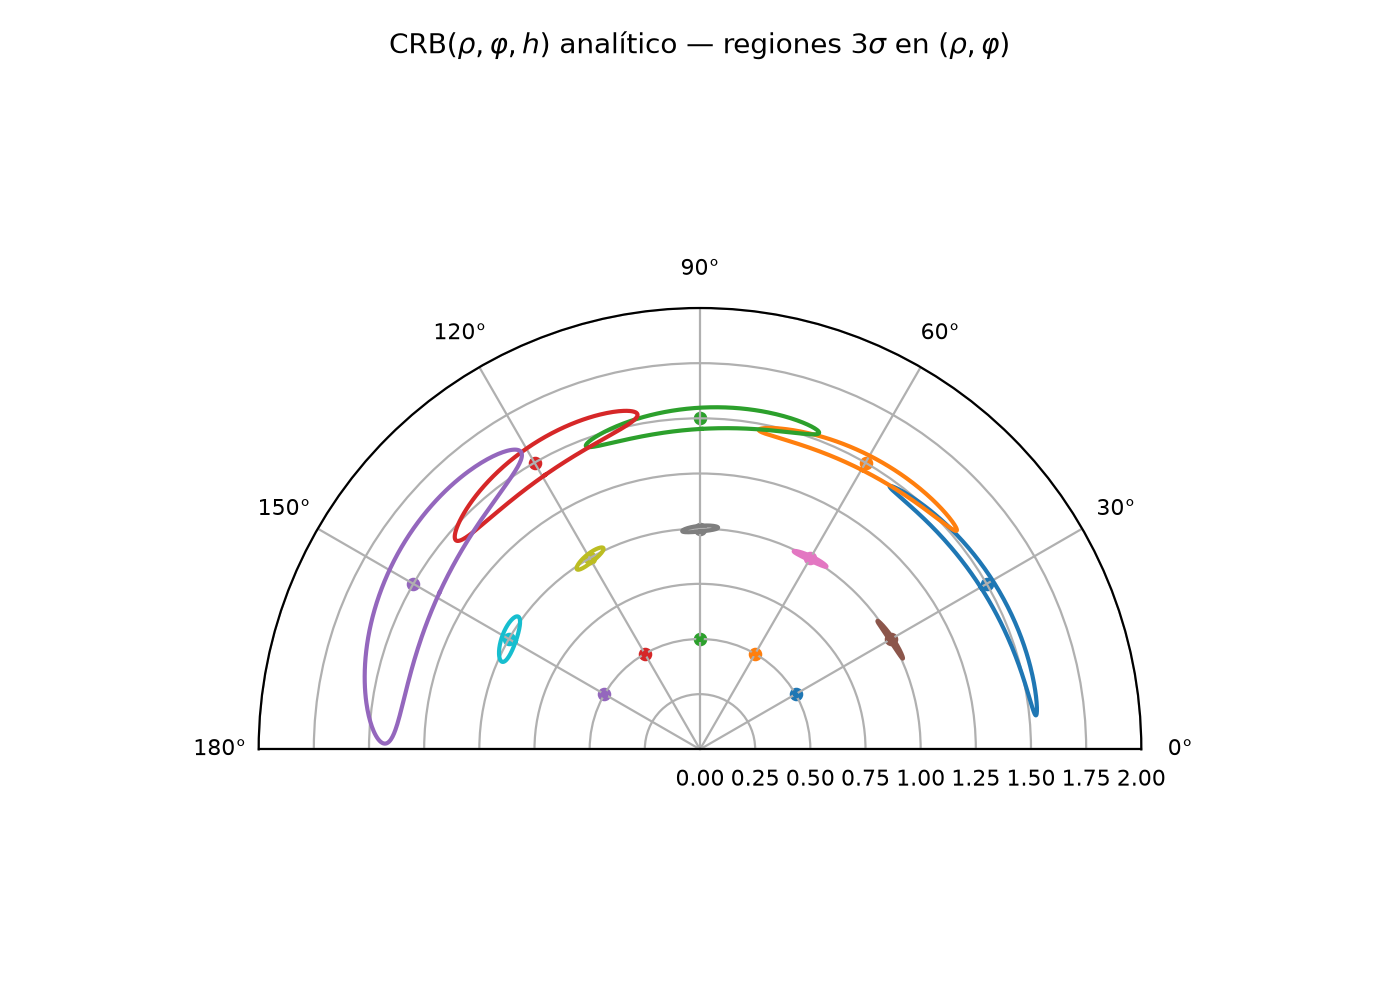
\includegraphics[width=0.86\textwidth]{../plots/crb_standard_regions_analytic.png}
\caption{CRB$(\rho,\varphi,h)$ \emph{anal\'itico}: regiones $3\sigma$ en
$(\rho,\varphi)$. Elipses (burbujas) generadas con derivadas cerradas.
Archivo \texttt{plots/crb\_standard\_regions\_analytic.png}.}
\label{fig:analytic-regions}
\end{figure}

\subsection{Superposici\'on anal\'itico vs FD}
Comparamos contra el m\'etodo rasterizado / diferencias finitas, cuyo grid se
carga de \texttt{plots/crb\_grid\_results.pkl} (generado por
\texttt{regenerate\_crb\_standard\_regions.py}). Las superposiciones usan el
grid FD disponible en la cache: aqu\'i el grid \emph{fixed\_h} de dos
par\'ametros $[\rho,\varphi]$, que da una comparaci\'on \textbf{apples-to-apples}
(ambos m\'etodos estiman los mismos dos par\'ametros); el grid \emph{with\_h} de
tres par\'ametros es an\'alogo. La leyenda de la Tabla~\ref{tab:avf} indica qu\'e
grid se us\'o.

\begin{remark}[Escalas no comparables]
Las \textbf{magnitudes absolutas} del CRB anal\'itico y del FD \textbf{no} son
directamente comparables: son \emph{modelos distintos} (faceta puntual
anal\'itica con ganancia $G=10^5$ y geometr\'ia fija, frente al render de malla
del simulador). Por eso mostramos dos superposiciones: (a) tal cual, y (b)
\emph{normalizada en forma} (escalando las semiejes de cada m\'etodo por un
factor com\'un para igualar su $\sigma_\rho$ mediana), que compara
\textbf{orientaci\'on y relaci\'on de aspecto} sin depender del tama\~no.
\end{remark}

\begin{figure}[ht]
\centering
\IfFileExists{../plots/crb_regions_analytic_vs_fd.png}{%
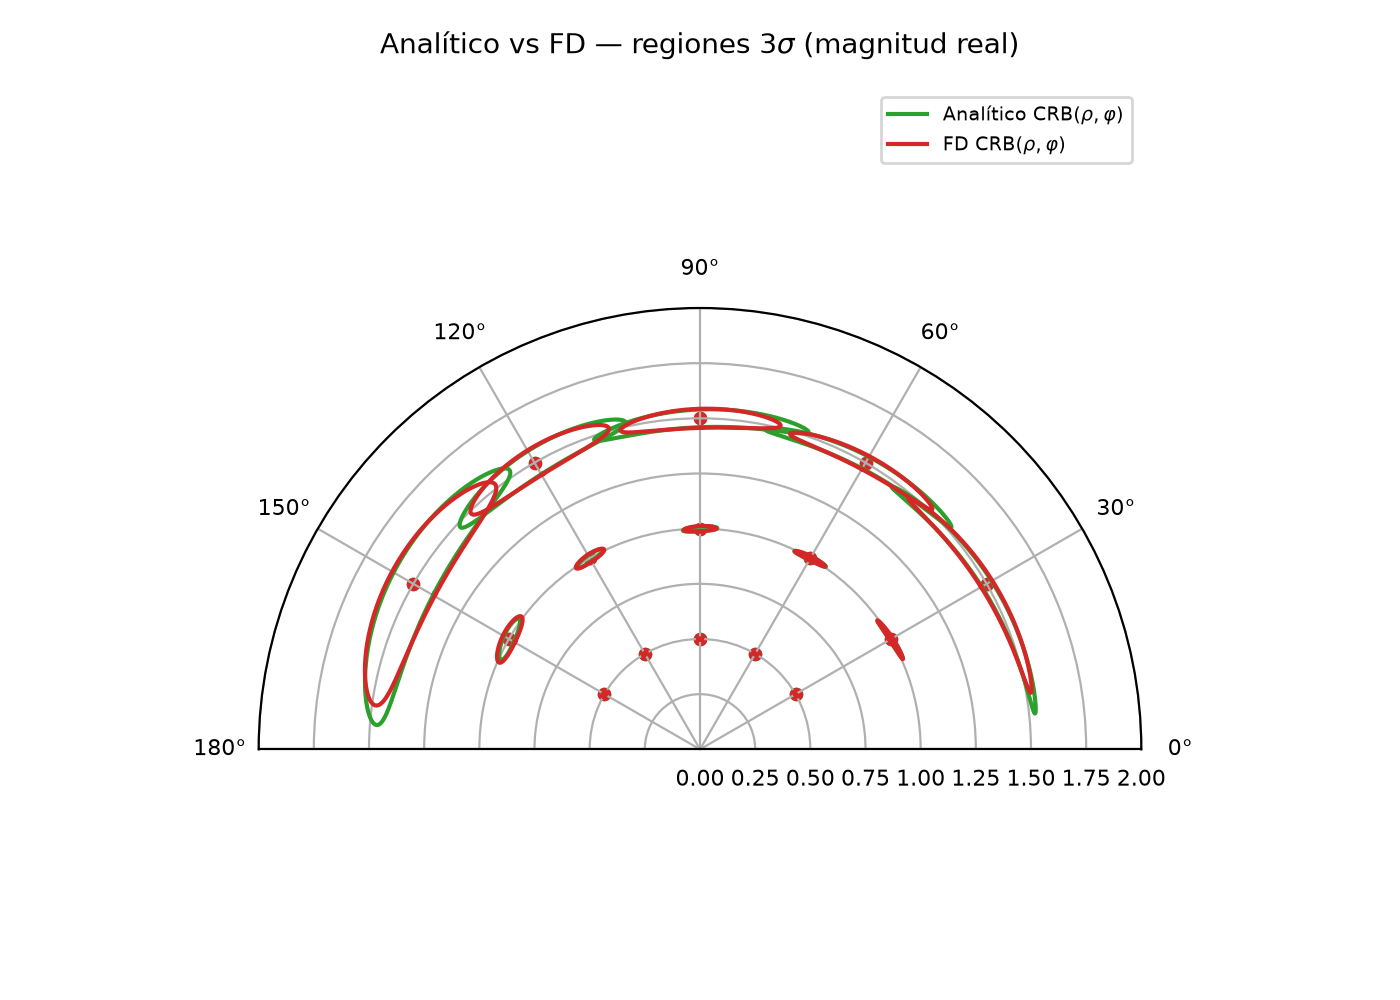
\includegraphics[width=0.72\textwidth]{../plots/crb_regions_analytic_vs_fd.png}%
}{\textit{(Pendiente: ejecutar la comparaci\'on con la cache FD disponible.)}}
\caption{(a) Superposici\'on anal\'itico (C2) vs FD (C3) a \emph{magnitud real}.
Archivo \texttt{plots/crb\_regions\_analytic\_vs\_fd.png}.}
\label{fig:avf-abs}
\end{figure}

\begin{figure}[ht]
\centering
\IfFileExists{../plots/crb_regions_analytic_vs_fd_shapenorm.png}{%
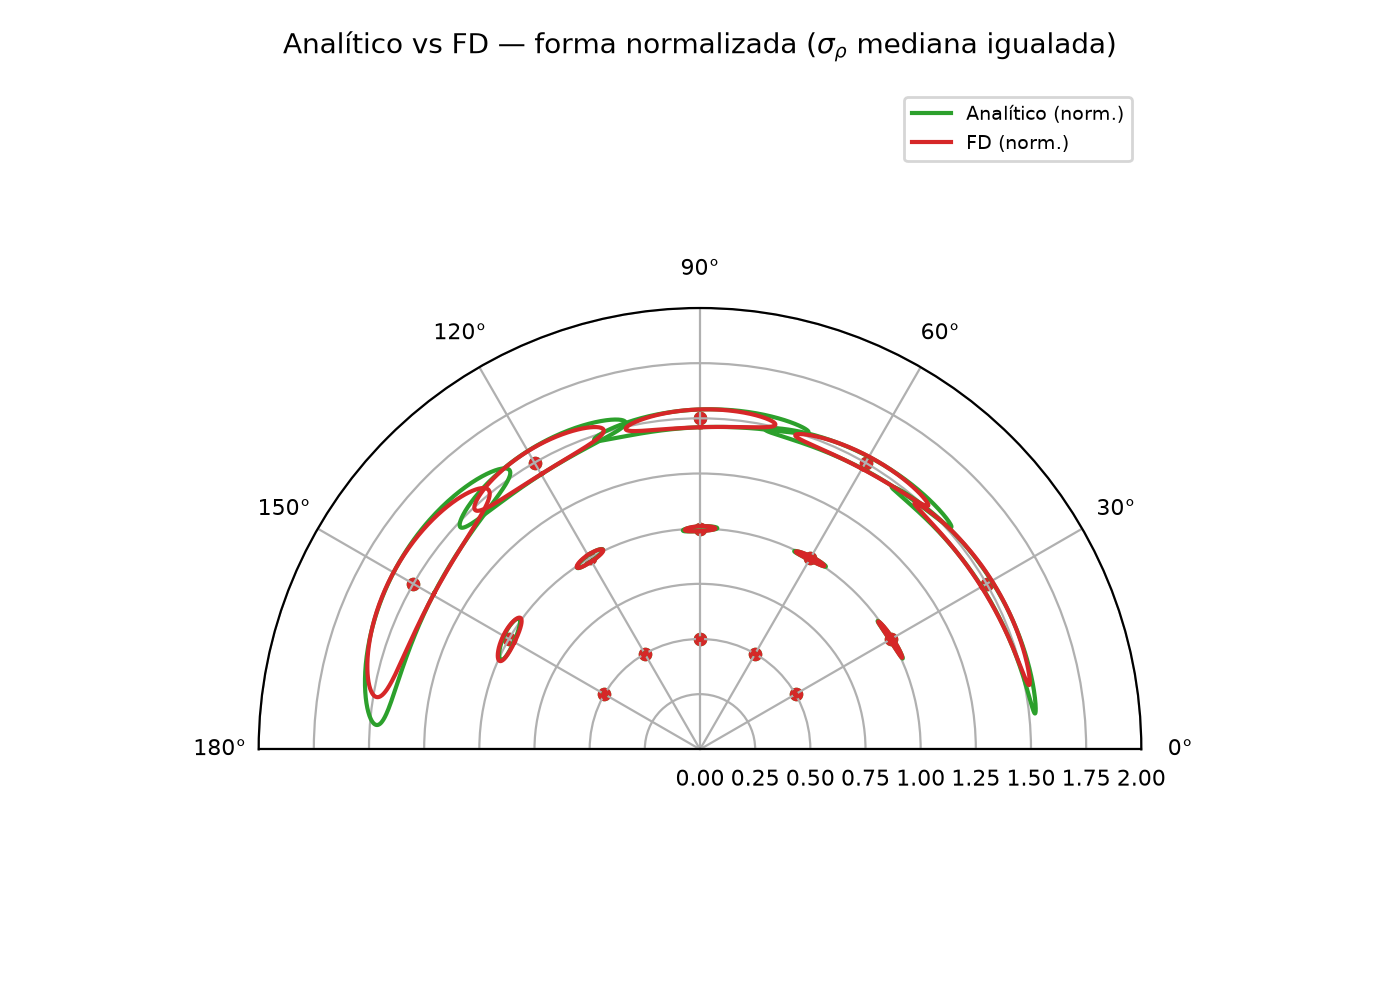
\includegraphics[width=0.72\textwidth]{../plots/crb_regions_analytic_vs_fd_shapenorm.png}%
}{\textit{(Pendiente: ejecutar la comparaci\'on con la cache FD disponible.)}}
\caption{(b) Superposici\'on \emph{normalizada en forma} ($\sigma_\rho$ mediana
igualada): compara orientaci\'on y aspecto de las elipses, no el tama\~no.
Archivo \texttt{plots/crb\_regions\_analytic\_vs\_fd\_shapenorm.png}.}
\label{fig:avf-shape}
\end{figure}

\subsection{Tabla num\'erica resumida}
La Tabla~\ref{tab:avf} resume, para el grid \emph{with\_h}, las desviaciones
$\sigma_\rho,\sigma_\varphi,\sigma_h$ y la \textbf{relaci\'on de aspecto}
(eje mayor/eje menor de la elipse $3\sigma$ en $(\rho,\varphi)$) de cada
m\'etodo; la tabla completa (incluida la inclinaci\'on \emph{tilt}) est\'a en
\texttt{docs/analytic\_vs\_fd\_comparison.txt}.

\IfFileExists{analytic_vs_fd_table.tex}{% Auto-generated by generate_analytic_crb_plots.py -- do not edit by hand.
\begin{table}[ht]
\centering\small
\caption{CRB anal\'itico vs FD sobre el grid $[\rho,\varphi]$ (\emph{fixed\_h}). $\sigma_\rho$ en m, $\sigma_\varphi$ en grados; \emph{asp}$=$eje mayor/menor de la elipse $3\sigma$ en $(\rho,\varphi)$. Magnitudes absolutas no comparables (modelos distintos); comparar \emph{asp} y la forma.}
\label{tab:avf}
\begin{tabular}{@{}rr|rrr|rrr@{}}
\toprule
 & & \multicolumn{3}{c|}{Anal\'itico} & \multicolumn{3}{c}{FD (rasterizado)} \\
$\rho$ & $\varphi^\circ$ & $\sigma_\rho$ & $\sigma_\varphi$ & asp & $\sigma_\rho$ & $\sigma_\varphi$ & asp \\
\midrule
0.5 & 30 & 0.005255 & 1.73 & 7.0 & 0.0006859 & 0.509 & 19.2 \\
0.5 & 60 & 0.004762 & 1.16 & 4.5 & 0.0006779 & 0.44 & 14.0 \\
0.5 & 90 & 0.005615 & 1.16 & 3.7 & 0.0007805 & 0.385 & 9.6 \\
0.5 & 120 & 0.008278 & 1.01 & 2.2 & 0.001116 & 0.412 & 7.1 \\
0.5 & 150 & 0.01454 & 1.46 & 1.8 & 0.001847 & 0.548 & 5.7 \\
1.0 & 30 & 0.005748 & 2.26 & 10.1 & 0.003406 & 2.01 & 13.1 \\
1.0 & 60 & 0.004987 & 1.57 & 6.3 & 0.003448 & 1.48 & 8.2 \\
1.0 & 90 & 0.00585 & 1.64 & 5.2 & 0.004197 & 1.42 & 6.2 \\
1.0 & 120 & 0.008383 & 1.42 & 3.0 & 0.006299 & 1.46 & 4.2 \\
1.0 & 150 & 0.01434 & 2.08 & 2.6 & 0.01086 & 2.21 & 3.7 \\
1.5 & 30 & 0.0102 & 4.11 & 11.2 & 0.01207 & 6.76 & 12.1 \\
1.5 & 60 & 0.00874 & 2.98 & 7.0 & 0.01215 & 4.69 & 7.2 \\
1.5 & 90 & 0.01025 & 3.31 & 6.1 & 0.01486 & 4.66 & 5.7 \\
1.5 & 120 & 0.01454 & 2.83 & 3.5 & 0.02185 & 4.72 & 3.8 \\
1.5 & 150 & 0.02478 & 4.28 & 3.0 & 0.03747 & 7.43 & 3.5 \\
\bottomrule
\end{tabular}
\end{table}
}{%
\textit{(Tabla pendiente: ejecutar \texttt{generate\_analytic\_crb\_plots.py}
con la cache FD disponible.)}}

\subsection{\textup{?`}Cu\'al elipse es ``mejor''?}
Aqu\'i ``mejor'' se refiere a la \textbf{calidad/suavidad de la derivada} y a la
\textbf{sensatez de la forma}, \emph{no} a la magnitud absoluta:
\begin{enumerate}[nosep]
    \item \textbf{Suavidad / condicionamiento.} El forward anal\'itico tiene
    derivadas \emph{exactas} ($C^\infty$). El Jacobiano FD se calcula sobre un
    forward con escalones (la cuantizaci\'on $\lceil\cdot\rceil$ y la m\'ascara
    $\texttt{xint}>0$ son constantes a trozos), de modo que la diferencia finita
    mezcla mesetas planas (derivada nula) con saltos de bin, introduciendo ruido
    de discretizaci\'on y dependencia del paso $\delta$. La elipse anal\'itica es
    la \textbf{mejor condicionada} (Fisher m\'as estable).
    \item \textbf{Forma / orientaci\'on.} Ambos m\'etodos dan elipses finas en
    \'angulo (resoluci\'on azimutal de la arista) y m\'as anchas en rango, f\'isicamente
    coherente; la orientaci\'on es consistente salvo el ruido FD.
    \item \textbf{Salvedad.} El modelo de faceta puntual \emph{no} reproduce el
    rasterizador; su CRB depende de $G,\beta,\kappa,\tau$ y de la geometr\'ia
    fija. La comparaci\'on honesta es de \emph{forma} (Fig.~\ref{fig:avf-shape}),
    no de tama\~no.
\end{enumerate}
\textbf{Veredicto:} para un CRB \emph{diferenciable}, la elipse \textbf{anal\'itica}
es preferible por derivadas exactas y Fisher mejor condicionada; el FD sigue
siendo valioso como verificaci\'on independiente y como modelo de malla completo.

%==============================================================================
\section{Conclusi\'on}
\label{sec:conclusion}
%==============================================================================

Partiendo del render rasterizado --- no diferenciable por
$\lceil\cdot\rceil$, umbral de ocultamiento y \emph{clamps} ---, construimos un
forward de faceta $C^\infty$ reemplazando cada discontinuidad por su an\'alogo
cerrado: la masa de Dirac en un bin por la \textbf{integral gaussiana}
\eqref{eq:erf-bin} (diferencia de $\erf$, el coraz\'on de la
diferenciabilidad), el Heaviside por una \textbf{sigmoide} \eqref{eq:sigmoid}, y
$\max(0,\cdot)$ por \textbf{softplus} \eqref{eq:softplus}. Con ello:
\begin{itemize}[nosep]
    \item las derivadas $\partial g/\partial\rho,\partial g/\partial\varphi,
          \partial g/\partial h$ son \textbf{exactas} y se obtienen
          simb\'olicamente (\texttt{sympy}), sin ajustar el paso $\delta$;
    \item $g_q$ y sus derivadas est\'an \textbf{bien definidas en $0$} gracias al
          fondo $b>0$, que hace innecesario el piso $\varepsilon$;
    \item la Fisher y el CRB \eqref{eq:fisher}--\eqref{eq:crb} conservan la
          estructura del \emph{writeup};
    \item la validaci\'on anal\'itico-vs-FD da error m\'aximo relativo
          $\sim5\times10^{-10}$.
\end{itemize}
La salvedad importante: este modelo anal\'itico de faceta puntual
\textbf{difiere} del rasterizador de malla, y sus valores de CRB dependen de la
ganancia $G$ y de los par\'ametros de suavizado $(\beta,\kappa,\tau)$, que
recuperan el l\'imite duro cuando $\beta,\kappa\to\infty$ y $\tau\to0$.

%------------------------------------------------------------------------------
\paragraph{Archivos.}
\texttt{crb\_analytic\_forward.py} (forward + Jacobiano simb\'olico + CRB),
\texttt{validate\_analytic\_forward.py} (validaci\'on anal\'itico vs FD),
este documento \texttt{docs/analytic\_forward\_crb.tex}.
Reutiliza (sin modificar) \emph{helpers} de \texttt{crb\_polar\_functions.py}.

\end{document}
